\subsection{Subjects}

Seven subjects, four women and three men, aged $30$ to $73$,
volunteered to join the experiment. They were all right-handed and
fully able-bodied, and were given no knowledge of the aim of the
experiment. Four of the subjects were slightly visually
impaired.

\subsection{Setup and devices}

The subjects were asked to sit confortably in front of a clean
workspace, and a flat $17$ inches color monitor was placed in front of
them at a distance of about half a meter. They wore an Immersion
\emph{CyberGlove} data glove \cite{cyberglove} on their right hand,
and an Ascension \emph{Flock-of-Birds} (FoB) \cite{fob} magnetic
tracker was firmly mounted on top of their wrist. Lastly, an ASL
\emph{E504} gaze tracker \cite{e504} was placed on the left hand side
of the monitor. Figure \ref{fig:devices} shows the devices and setup.

\begin{figure*}[ht]
  \centering
    \begin{tabular}{ccc}
      \includegraphics[width=0.295\linewidth]{figs/glove.eps} &
      \includegraphics[width=0.295\linewidth]{figs/e504.eps} &
      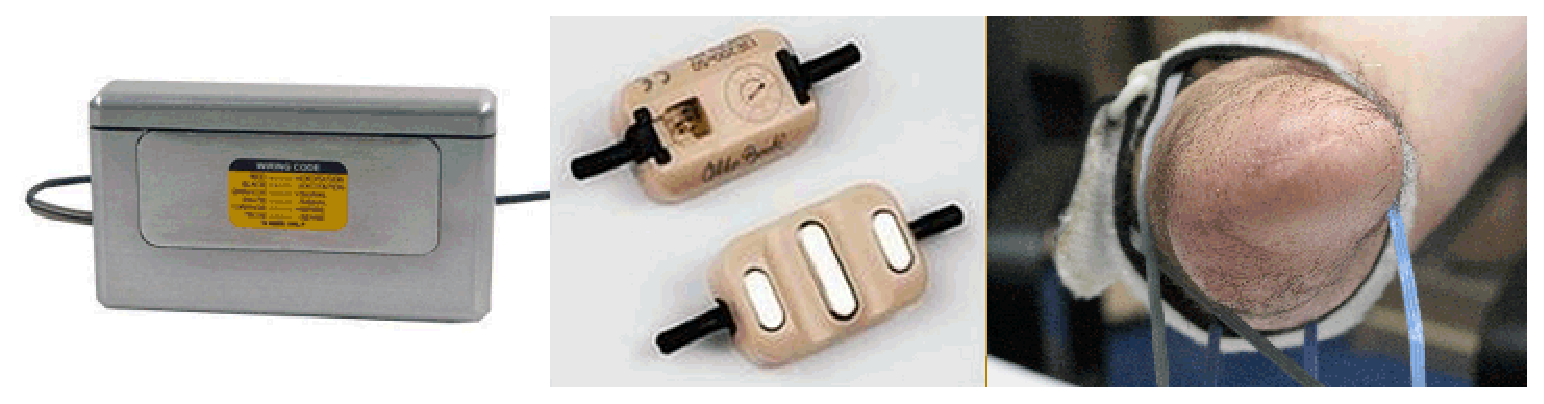
\includegraphics[width=0.295\linewidth]{figs/setup.eps} \\
      $(a)$ & $(b)$ & $(c)$
    \end{tabular}
    \caption{The setup and devices used for the experiment: $(a)$ the
    Immersion CyberGlove with the Flock-of-Birds sensor just above the
    wrist; $(b)$ the ASL E504 gaze tracker (pan/tilt near-infrared
    camera); $(c)$ the whole setup.}
    \label{fig:devices}
\end{figure*}

The FoB returns six double-precision numbers describing the position
($x$, $y$ and $z$ in inches) and rotation (azimuth, elevation and roll
in degrees) of the sensor with respect to a magnetic basis mounted
about one meter away from the subject. Its resolution is $0.1$ inches
and $0.5$ degrees. The E504, after a careful calibration phase,
returns one true/false value, denoting validity of the gaze
coordinates, and two double-precision numbers indicating the
coordinates of the subject's gaze with respect to the monitor. The
CyberGlove was used as an on-off switch, to detect when the subject's
hand would close, by monitoring one of its sensors via a threshold.

The monitor showed the slave's workspace; the slave is the humanoid
platform Babybot \cite{babybotHum2005}. For the experiment we only
employed one of its colour cameras.

All data were collected, synchronised, and saved in real time at a
frequency of about $47$Hz.

\subsection{Method}

The subjects were asked to initially keep their right hand and arm in
a resting position. The monitor showed the slave's workspace, in which
several objects could be clearly seen, and a moving red cross
corresponding to the detected subject's gaze. The subjects were then
instructed, upon a request by the experimenter, to look at one of the
objects on the monitor and then to move their hand as if to reach and
grasp it, signalling the act of grasping by closing their right
hand. The red cross on the screen turned green when the hand was
closed, to confirm the grasping.

This fake grasping act was repeated for $15$ to $21$ times, each time
with a different object (therefore, toward a different position) seen
on the monitor. The maximum duration of the whole experiment for a
single subject was about $3.5$ minutes, resulting in no tiredness.

\subsection{Building the data set}
\label{subsec:dataset}

The first question was \emph{what} to monitor from the subjects'
data. A few intuitive considerations led us to consider $(a)$ the
average of the subjects' hand velocity, $(b)$ the variance of the
subjects' gaze coordinates and $(c)$ the information whether the
subjects' right hand was open or closed. When the subject wants to
grasp an object, he/she first \emph{fixates} the desired object and
then \emph{reaches} for it (see, e.g., \cite{johansson01}); lastly, at
some time after the beginning of the reaching movement, he/she will
close the right hand as if to grasp, as instructed.

We then expect, while fixating, the gaze coordinates to hover around
the point on the screen where the desired object is seen, that is,
their standard deviation over some time to be \emph{small}; also we
expect, while reaching, the hand to move toward the object on the
screen, that is, the hand velocity components to be on average
\emph{large}. The instants in which the hand is closed will signal the
intention to grasp, whereas those when the hand is open will be taken
as negative examples. Data $(a)$ were easily obtained by
differentiating in time the hand position $x,y,z$ coordinates obtained
from the FoB, while $(b)$ and $(c)$ were obtained straight from the
E504 and the CyberGlove. (The samples corresponding to negative values
of the E504 validity flag were ignored, manually verifying that this
would not hamper the overall statistics.)

From each subject we obtained a sequence of $6$-tuples (the three hand
velocity coordinates, the two gaze coordinates and the open/closed
hand flag). The above considerations should be valid \emph{over a
certain time window}, characteristic of the fixation/reaching
operations --- call it $\tau$; and in general each subject will have a
different $\tau(i), i=1,\ldots,7$. Driven by this, we then decided to
feed the learning system the following data: for each user $i$ (and
therefore for each sequence) and for a range of different values $T_c$
attributed to $\tau(i)$, the \emph{hand velocity average values} over
$T_c$ (three real numbers) and the \emph{gaze position standard
deviations} over $T_c$ (two real numbers). Training was enforced by
requiring that the the system could guess, instant by instant, whether
the hand was closed or not. This was represented as an integer value,
in turn $1$ or $-1$. The problem of guessing when the subject wants to
grasp was thus turned into a typical supervised learning problem.

\subsection{Grasping speed}

In choosing the range for $T_c$, we were driven by the main
consideration that a moving time window should not be longer then the
interval of time between one grasping attempt and the following
one. In fact, a longer time window could trick the system into
considering data obtained during two or more independent grasping
attempts.

By examining all sequences we found out that the interval between one
grasping attempt and the following one lasted on average $7.1 \pm 1.8$
seconds. We then decided to let $T_c$ range in the interval
$0.1,\ldots,5$ seconds.

In general, we expected to find a best minimum value for $T_c$, which
would then be the required $\tau(i)$ for each user, figuring out that
shorter values would convey too little information about the ongoing
movement, and that for longer ones, the moving averages would reach a
plateau effect, tending to the overall average values of the hand
velocity and gaze standard deviations.

\subsection{Support Vector Machines}
\label{subsec:svm}

Our machine learning system is based upon Support Vector Machines
(SVMs). Introduced in the early 90s by Boser, Guyon and Vapnik
\cite{BGV92}, SVMs are a class of kernel-based learning algorithms
deeply rooted in Statistical Learning Theory \cite{v-edbed-82}, now
extensively used in, e.g., speech recognition, object classification
and function approximation with good results \cite{Cristianini00}. For
an extensive introduction to the subject, see, e.g., \cite{Burges98}.

We are interested here in the problem of SVM classification, that is:
given a set of $l$ training samples $S=\{\xx_i,y_i\}_{i=1}^l$, with
$\xx_i \in \RR^m$ and $y_i \in \{-1,1\}$, find a function $f$, drawn
from a suitable functional space $\mathcal{F}$, which best
approximates the probability distribution of the source of the
elements of $S$. This function will be called a \emph{model} of the
unknown probability distribution. In order to decide whether a sample
belongs to either category, the sign of $f$ is considered, with the
convention that $sgn(f(\xx)) \geq 0$ indicates $y = 1$ and
vice-versa. In practice, $f(\xx)$ is a sum of $l$ elementary functions
$K(\xx,\yy)$, each one centered on a point in $S$, and weighted by
real coefficients $\alpha_i$:

\begin{equation} \label{eqn:sol}
  f(\xx) = \sum_{i=1}^l \alpha_i K(\xx,\xx_i) + b
\end{equation}

\noindent where $b \in \RR$. The choice of $K$, the so-called
\emph{kernel}, is done \emph{a priori} and defines $\mathcal{F}$ once
and for all; it is therefore crucial. According to a standard practice
(see, e.g., \cite{Cristianini00}) we have chosen a \emph{Gaussian}
kernel, which has one positive parameter $\sigma \in \RR$ which is the
standard deviation of the Gaussian functions used to build
(\ref{eqn:sol}). Notice that this is not related to the fact that the
target probability distribution might or might not be Gaussian.

Now, let $C \in \RR$ be a positive parameter; then the $\alpha_i$s and
$b$ are found by solving the following minimisation problem
(\emph{training phase}):

\begin{equation} \label{eqn:svm_primal}
  \arg \min_{\aa} \left( R(S,K,\aa) + C \sum_{i=1}^l L(\xx_i,y_i,f) \right)
\end{equation}

\noindent where $R$ is a \emph{regularisation term} and $L$ is a
\emph{loss functional}. In practice, after the training phase, some of
the $\alpha_i$s will be zero; the $\xx_i$s associated with non-zero
$\alpha_i$s are called \emph{support vectors}. Both the training time
(i.e., the time required by the training phase) and the testing time
(i.e., the time required to find the value of a point not in $S$)
crucially depend on the total number of support vectors; therefore,
this number is an indicator of how hard the problem is. Since the
number of support vectors is proportional to the sample set
\cite{Steinwart03}, an even better indicator of the hardness of the
problem is the percentage of support vectors with respect to the
sample set size. We will denote this percentage by the symbol $p_{SV}$
and call it \emph{size} of the related model. Willing to implement the
system on-line, one has to choose models with the smallest possible
size.

In (\ref{eqn:svm_primal}), minimising the sum of $R$ and $L$ together
ensures that the solution will approximate well the values in the
training set, at the same time avoiding overfitting, i.e., exhibiting
poor accuracy on points outside $S$. Smaller values of the parameter
$C$ give more importance to the regularisation term and vice-versa.

There are, therefore, two parameters to be tuned in our setting: $C$
and $\sigma$. In all our tests we found the optimal values of $C$ and
$\sigma$ by grid search with $3$-fold cross-validation. This ensures
that the obtained models will have a high generalisation power, i.e.,
their guess will be accurate also on samples not in $S$.

Notice, lastly, that the quantity to be minimised in Equation
(\ref{eqn:svm_primal}) is convex; due to this, as well as to the use
of a kernel, SVMs have the advantages that their training is
guaranteed to end up in a global solution and that they can easily
work in highly dimensional, non-linear feature spaces, as opposed to
analogous algorithms such as, e.g., artificial neural networks. As a
matter of fact, SVMs are best employed when the chosen kernel maps the
samples to a space in which the problem is \emph{linearly separable},
that is, a hyperplane (linear function) can be found which separates
the samples labelled $1$ from those labelled $-1$.

We have employed LIBSVM v2.82 \cite{ChangL01}, a standard, efficient
implementation of SVMs.

According to the procedure described in the previous parts of this
Section, we decided to set up a SVM for each user $i$ and value of the
time window $T_c$. Willing to compare the performance with and wothout
the use of the gaze signal, we defined $\RR^{3}$ as the input space in
the case of not using the gaze (the $3$ numbers representing the hand
average velocity over $T_c$), and $\RR^{5}$ in the case of using the
gaze (the $5$ numbers representing the hand velocity average and gaze
position standard deviation over $T_c$). According to this and to the
experience gathered in previous work \cite{clea07}, the ranges of the
parameters $C$ and $\sigma$ were chosen as follows: $C$ was $10^k$
with $k=-1,\ldots,3$ in steps of $0.2$, whereas $\sigma$ was
$\sqrt{\frac{5}{10^{k}}}$ with $k=0,\ldots,2$, in steps of $0.2$.
